\section{Preliminaries and Related Work}
\label{sec:preliminaries}

\paragraph*{On Sampling Strategies.}
\label{ssec:sens_sampling}

As discussed, we focus our study on linear- and sublinear-time sampling strategies. Specifically, given a dataset $P \in \R^{n \times d}$, we want to sample
$\Omega \in \R^{m \times d} \subset P$ such that $m \ll n$ along with a weights vector $w \in \R^m$. The goal is then that for some solution $\calC$, $\Omega$
provides us with an idea of the solution's quality with respect to the original dataset, i.e. $\sum_{p \in \Omega} w_p \cost(p, \calC) \sim \sum_{p \in P}
\cost(p, \calC)$.  The quickest sampling strategy, running in sublinear time, is uniform sampling. It is clear, however, that this cannot provide any
cost-preservation guarantee as missing a single extreme outlier will cause the sampling strategy to fail. Thus, any approach that outperforms this strategy must
read in the entire dataset and therefore run in at least linear time. Indeed, sublinear algorithms always require some assumption on the input to provide
guarantees, see \cite{Ben-David07,czumaj2007sublinear,HJJ23,meyerson2004k}.


Among these more sophisticated sampling strategies, coresets offer the strongest compression guarantee. Specifically, a strong $\eps$-coreset is an 
$\Omega
\subseteq P$ with weights $\tilde w$ such that for \emph{any} solution $\calC$, \[\sum_{p \in \Omega} \tilde w_p \cost(p, \calC) \in (1 \pm \eps) \cost(P, \calC)\] with
high probability.  Going forward, we will discuss this in the context of the $k$-median and $k$-means cost functions: for dataset $P \in \R^d$ with weights $w
: P \rightarrow \R^+$, and any $k$-tuple $\calC$ in $\R^d$, \[\cost_z(P, \calC) := \sum_{p \in P} \tilde w(p) \dist^z(p, \calC),\] with
$z=1$ for $k$-median and $z=2$ for $k$-means. We use $\opt$ to denote $\min_{\Omega} \cost_z(P, \calC)$.

Recently, sampling with respect to sensitivity values has grown to prominence due to its simplicity and coreset guarantee.  True sensitivity values are defined
as $\sup_{\calC} \frac{\dist^z(p, \calC)}{\cost_z(P, \calC)}$, where the supremum is taken over all possible solutions $\calC$. Intuitively, this is a measure
of the maximum impact a point can have on a solution and is difficult to evaluate directly.
Thus, the approximate sensitivity-sampling algorithm we consider is the following, as introduced in \cite{FeldmanL11}.
Given an $\alpha$-approximate solution to a clustering problem $\calC$, importance scores are defined as
\begin{equation}
\label{eq:sensitivity}
\sigma_\calC(p) = \alpha \cdot \left( \dfrac{\cost(p, \calC)}{\cost(\calC_{p}, \calC)} + \dfrac{1}{|\calC_p|} \right),
\end{equation}
where $\calC_p$ is the cluster that $p$ belongs to. This is always an upper-bound on the sensitivity values, see \cite{FL11,FeldmanSS20}.

The coreset $\Omega$ then consists of $m$ points sampled proportionate to $\sigma$ with weights defined as follows. First, for any sampled point $p$, define $w_p :=
\frac{1}{\Pr[p \in \Omega]} = \frac{\sum_{p'} s_\calC(p')}{m s_\calC(p)}$. For a cluster $C_i$, let $|\hat{C_i}|$ be the number of points in $C_i$ estimated by the
sample, i.e. $C_i \cap \Omega$ weighted with $w_p$. A sampled point $p$ in $C_i$ is
weighted $\tilde w(p) = \tilde w_1(p) \lpar (1+\eps)|C_i| - |\hat{C_i}|\rpar$.  \cite{FeldmanL11} and subsequent works showed that, when $\calC$ is
a $O(1)$-approximation, sampling $\Omega = \tilde O\lpar k \eps^{-2z-2}\rpar$ many points was enough to ensure concentration, namely, $\Omega$ is a coreset with
probability at least $2/3$.

To perform this algorithm, the bottleneck in the running time lies in computing the solution $\calC$ as well as then obtaining costs of every point to its
assigned center in $\calC$. Using any bicriteria approximation algorithm\footnote{For $k$-means an $(\alpha,\beta)$ bicriteria approximation is an algorithm
that computes a solution $\calC$ satisfying $\cost(P\calC)\leq \alpha\cdot \opt$ and $|\calC|\leq \beta\cdot k$.} such as the standard $k$-means++ algorithm
\cite{ArV07} combined with dimension reduction techniques (see for example \cite{BecchettiBC0S19,CohenEMMP15,MakarychevMR19}), this takes time $\tilde O(nk
+nd)$. This is precisely what was conjectured as the necessary runtime for obtaining $k$-means and $k$-median coresets, as merely assigning points to their
centers from the bicriteria seems to require $\Omega(nk)$ running time.

\begin{figure*}
\label{fig:coreset_size_on_sens_quality}
\centering
\begin{tabular}{lc}
    \rotatebox[origin=l]{90}{\bf \;\quad\quad\quad\quad\quad\quad\quad$k$-Median} &
    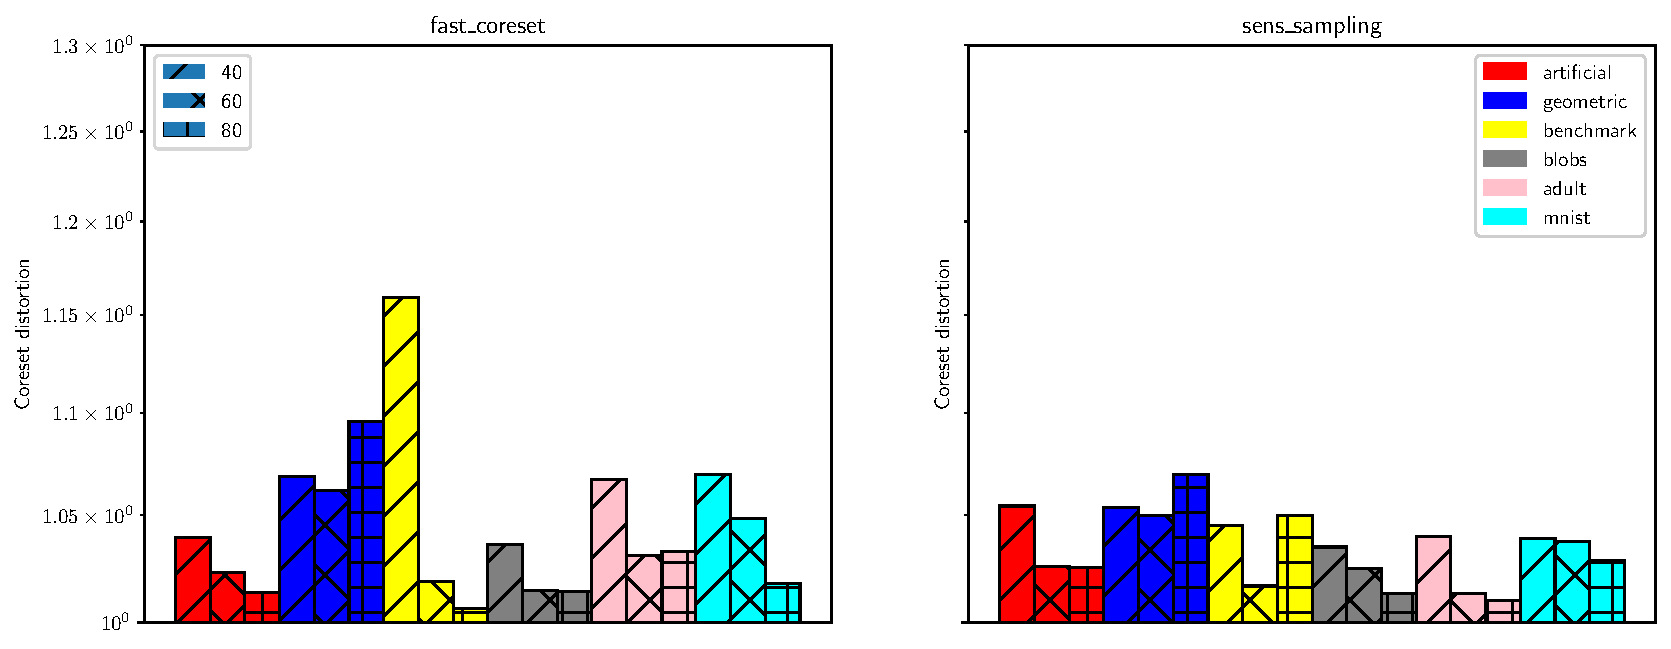
\includegraphics[width=.95\linewidth]{images/1/coreset_distortion-m_scalar_for_sens_sampling.pdf} \\

    \rotatebox[origin=l]{90}{\bf \;\;\quad\quad\quad\quad\quad\quad\quad$k$-Means} &
    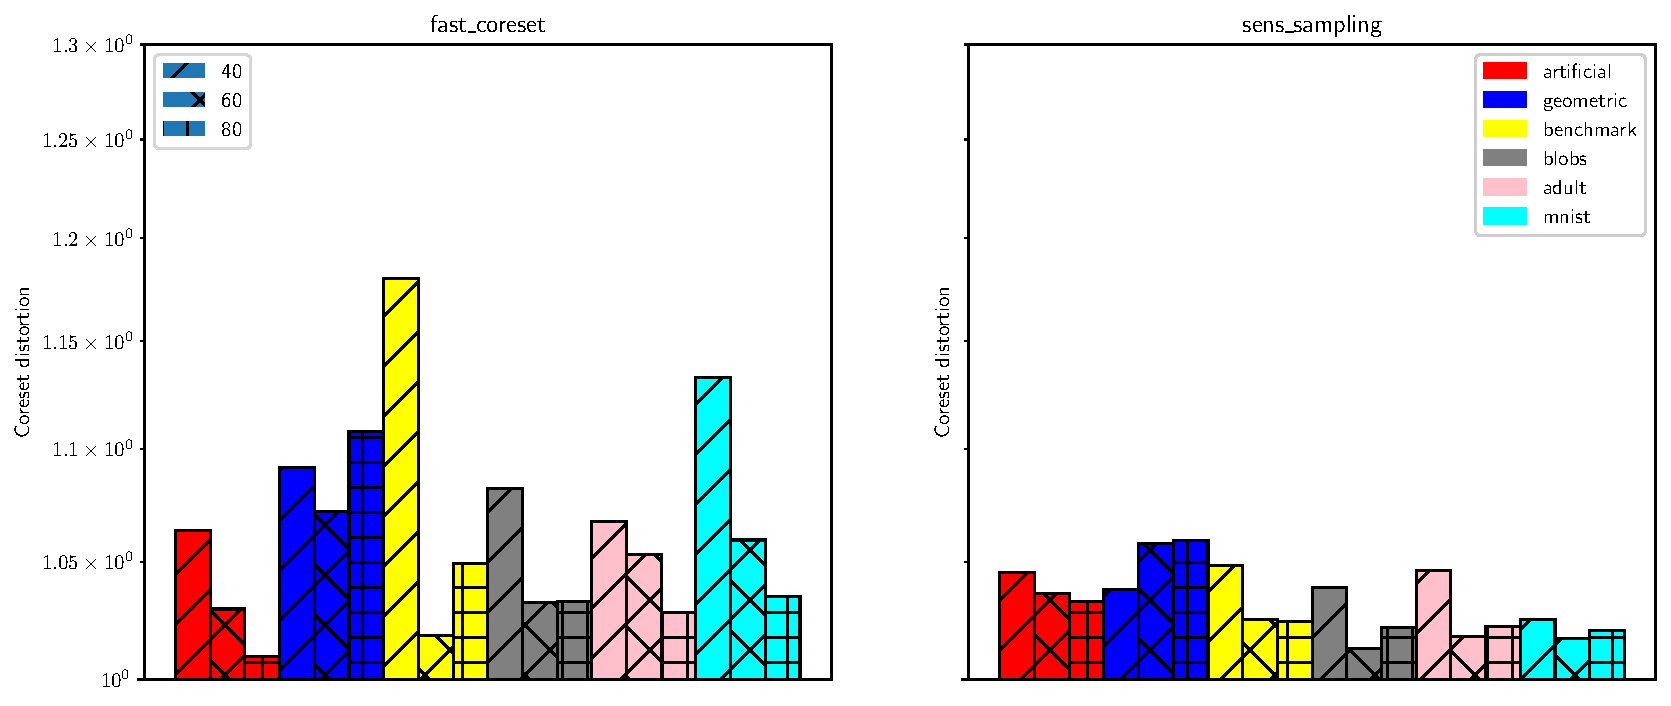
\includegraphics[width=.95\linewidth]{images/2/coreset_distortion-m_scalar_for_sens_sampling.pdf}
\end{tabular}
\caption{The effect of the coreset size on the distortion metric for sensitivity sampling approaches.
We point out that all distortion values are well below $\varepsilon = 0.2$.
Thus, for sufficient coreset sizes, there does not seem to be a meaningful difference between using Fast-Kmeans++ vs. regular Kmeans++.}
\end{figure*}


\paragraph*{Other Coreset Strategies}
\label{ssec:clustering_prelim}

Much of the advancements regarding coresets have sought the smallest coreset possible across metric spaces and downstream objectives. The most prominent
examples are in Euclidean space \cite{BadoiuHI02, HaM04, Chen09, HuangV20, stoc22}, with much of the focus on obtaining the optimal size in the $k$-means and
$k$-median setting. Recently, a lower bound \cite{huangLB} showed that the group sampling algorithm developed in \cite{stoc21, stoc22} is optimal.

Although this algorithm's coresets have size $\tilde{O}(k\cdot \varepsilon^{-2} \min(k^{z/(z+2)},\varepsilon^{-z}))$ \cite{CLSSS22} and are theoretically smaller than
those obtained by sensitivity sampling, the experiments of \cite{chrisESA} showed that the latter is often more efficient in practice. We also note that one
could use virtually any coreset construction as many are linear-time once provided with an initial solution $\calC$ and assignment $\sigma$.

In terms of other linear-time methods with sensitivity sampling, we are only aware of the lightweight coresets approach (\cite{BachemL018}), wherein one
samples with respect to a solution $\calC=\{\mu\}$, i.e. the mean of the data set. This runs in $O(nd)$ time but provides a weaker guarantee -- one incurs an
additive error of $\varepsilon\cdot \cost(P,\{\mu\})$.  We note that this can be generalized to performing sensitivity sampling using a $\calC$ that has fewer
than $k$ centers. We discuss this in more depth in Section \ref{ssec:algorithms}.

All efficient coreset constructions are probabilistic and this comes with a disadvantage of coresets being difficult to evaluate. For example, it is co-NP-hard to
check whether a candidate compression is a weak coreset \footnote{A weak coreset guarantee only requires that a $(1+\varepsilon)$ approximation
computed on the coreset yields a $(1+\varepsilon)$ on the entire point set \cite{chrisESA}.}. Therefore, although coreset algorithms succeed with some high probability, it is
unclear how to computationally verify this. We refer to \cite{chrisESA} for further discussion on this topic and discuss our metrics in Section \ref{sssec:metrics}.

\paragraph*{Quadtree Embeddings}

To design fast algorithms, one of the common techniques is to embed the Euclidean space into a tree metric.  We give a brief description of the quadtree metric
embedding procedure here and refer to \cref{app:quadtree} for a more formal explanation.  The central idea is that each hypercube in the input space can be
split into $2^d$ sub-cubes and that this can be represented in a tree structure. Setting the weight of each branch equal to the length of the parent node's
diagonal then guarantees that the expected distance in the tree is within a factor $O(\sqrt{d} \log \Delta)$ of the distance in the original space, where
$\Delta$ is the \emph{spread} of the point set, namely the ratio of the largest distance by the smallest non-zero distance. Lastly, this tree can be constructed
in $\tilde{O}(nd \log \Delta)$ time.
